\documentclass{DeustoFDP}

\usepackage{hologo} % Paquete no necesario. Borrar en la memoria final al sustituir el texto
\usepackage{eurosym}
\usepackage{color}
\usepackage{placeins}
\usepackage{tikz}
\usepackage[toc, acronym, nomain]{glossaries}

\usetikzlibrary{matrix}

\setlength{\headheight}{12.22504pt}

\hypersetup{
  pdfauthor={Santiago Mazagatos Pérez Sebastian Rengel},
  pdftitle={Diseño e implementaci\'on de un Smart Mirror multiusuario con autenticaci\'on por reconocimiento facial},
}

\colorlet{helpful}{lime!70}
\colorlet{harmful}{red!30}
\colorlet{internal}{yellow!20}
\colorlet{external}{cyan!30}
\colorlet{F}{helpful!50!internal}
\colorlet{D}{harmful!50!internal}
\colorlet{O}{helpful!50!external}
\colorlet{A}{harmful!50!external}

\newcommand{\texta}{Beneficioso\par}
\newcommand{\textb}{Dañino\par}
\newcommand{\textcn}{Origen interno\par}
\newcommand{\textdn}{Origen externo\par}

\newcommand{\back}[1]{\fontsize{60}{70}\selectfont #1}

\bibliography{bibliografia}
\makeglossaries

\begin{document}

\newacronym{xml}{XML}{Extensible Markup Language}
\newacronym[longplural={Bases de Datos}]{bd}{BD}{Base de Datos}
\newacronym{http}{HTTP}{Hypertext Transfer Protocol}
\newacronym{api}{API}{Application Programming Interface}
\newacronym{html}{HTML}{HyperText Markup Language}
\newacronym{css}{CSS}{Cascading Style Sheets}
\newacronym{sql}{SQL}{Structured Query Language}
\newacronym{url}{URL}{Uniform Resource Locator}
\newacronym{edt}{EDT}{Estructura de Descomposición del Trabajo}
\newacronym{mvc}{MVC}{Modelo Vista Controlador}
\newacronym{json}{JSON}{JavaScript Object Notation}
\newacronym{uwp}{UWP}{Universal Windows Platform}
\newacronym{ces}{CES}{Consumer Electronics Show}
\newacronym{iot}{IoT}{Internet of Things}
\newacronym{paas}{PaaS}{Platform as a Service}
\newacronym{iaas}{IaaS}{Infraestructure as a Service}
\newacronym{xhtml}{XHTML}{Extensible Hyertext Markup Language}
\newacronym{xslt}{XSLT}{Extensible Stylesheet Language}
\newacronym{vb.net}{VB.NET}{Visual Basic .NET}
\newacronym{cppcli}{C++/CLI}{C++ modified for Common Language Infraestructure}
\newacronym{https}{HTTPS}{Hypertext Transfer Protocol Secure}
\newacronym{xaml}{XAML}{Extensible Application Markup Language}
\newacronym{risc}{RISC}{Reduced Instruction Set Computing}
\newacronym{arm}{ARM}{Advanced \acrshort{risc} Machine}
\newacronym{qr}{QR}{Quick Response}
\newacronym{sdk}{SDK}{Software Development Kit}
\newacronym{usb}{USB}{Universal Serial Bus}
\newacronym{gps}{GPS}{Global Positioning System}
\newacronym{wifi}{Wi-Fi}{Wireless Fidelity}
\newacronym{ai}{AI}{Application Insights}

\frontmatter 
\pagestyle{plain}

% Las siguientes lineas (21--26) se pueden eliminar del documento final.
% Notese que en ese caso es necesario descomentar la linea 28 para que las
% paginas esten correctamente numeradas.
\begin{titlepage} 
  \newgeometry{left=0cm,right=0cm,bottom=0cm,top=0cm}
  
\includegraphics{fig/portada_final}
  \restoregeometry
\end{titlepage}
\cleardoublepage

%\setcounter{page}{3}

\chapter*{Resumen}

El proyecto consistirá de una Raspberry Pi 2 Model B con Windows 10 IoT Core y un servidor en la plataforma Azure de Microsoft, la Raspberry mostrará datos generales como el tiempo o datos dependientes del usuario tales como sus emails sin leer, sus tareas y sus eventos de calendario y determinará el usuario haciendo uso de una WebCam y Project Oxford para reconocimiento facial.

Los usuarios dispondrán de una interfaz Web para entrar en su cuenta Google y autorizar al Smart Mirror para acceder a sus datos, asimismo, el servidor que hospeda la interfaz web se encargará de recoger la información de las diferentes API (Google Mail, Google Tasks, Google Calendar, el tiempo, Project Oxford) y suministrársela al espejo cliente.

Debido al planteamiento de la solución se pueden añadir más smart mirror sin que ningún usuario tenga que volver a configurar nada, y serán reconocidos por cualquier smart mirror siempre y cuando todos usen el mismo servidor como base.
La Raspberry tendrá, aparte de la pantalla y la WebCam un circuito electrónico con un interruptor cinético sensible que se activará al dar un toque al marco del smart mirror, todos los componentes estarán encapsulados en un marco con un espejo de dos caras que dejará pasar la luz de la pantalla al otro lado, mostrando la información al usuario en la superficie reflectante.


\vspace{2em}

{\Large\bfseries\sffamily Descriptores}
\vspace{3\medskipamount}

Smart Mirror, ASP.NET, \acrshort{iot}, \acrshort{uwp}.

\cleardoublepage\tableofcontents
\cleardoublepage\listoffigures
\cleardoublepage\listoftables
\cleardoublepage\lstlistoflistings

\mainmatter
\pagestyle{phdthesis}

\chapter{Introducción}\label{cha:introduccion}

\section{Presentación del documento}

El presente informe describe el proyecto de desarrollo \emph{Diseño e implementación de un Smart Mirror multiusuario con autenticación por reconocimiento facial}, cuyo objetivo es crear un Smart Mirror en el que cualquier usuario pueda ver información sobre su perfil online de forma rápida y sencilla, también se incluye una definición de objetivos, fases, actividades y recursos del proyecto.

El contenido de este documento se estructura en torno a los siguientes puntos.

\begin{itemize}
	\item \textbf{Objetivos del proyecto:}

	Definición general del proyecto y detalle de sus objetivos.

	\item \textbf{Especificación de requisitos:}
		
	Idea general del software a desarrollar asi como informacion sobre su funcionalidad y sus requisitos tanto funcionales como no funcionales.
	
	\item \textbf{Tecnologías utilizadas:}
		
	Información sobre todas las tecnologías que el software implementado va a usar.
	
	\item \textbf{Especificación del diseño:}

	Definición del código a implementar en la solución software.

	\item \textbf{Consideraciones sobre la implementación:}
	
	Descripción de aspectos importantes para la codificación del software.

	\item \textbf{Plan de pruebas:}

	Definición el proceso de verificación del software.

	\item \textbf{Manual de usuario:}
	
	Guia para el uso correcto del software.

	\item \textbf{Incidencias:}
	
	Problemas surgidos durante el desarrollo del proyecto y su solución.

\end{itemize}

\section{Motivación}

Este proyecto nace de la necesidad de un dispositivo que pueda mantener a un usuario conectado con su vida online, sin resultar una distracción para el mismo, por tanto, se procedió al diseño de una solución que fuera capaz de mostrar información relevante para el usuario sin necesidad de interacción excesiva por su parte, siendo solo necesaria una configuración inicial.

\section{El concepto de Smart Mirror}

Un Smart Mirror suele estar compuesto fundamentalmente de un monitor situado detrás de un espejo de observación de dos caras, de tal manera que la luz del monitor sea lo único que se vea sobre la superficie reflectante, creando una ilusión de que el contenido del monitor está plasmado en la superficie de un espejo normal y corriente, la función del Smart Mirror es proporcionar información útil para el usuario y en algunos casos, interacción sin necesidad de dispositivos adicionales como un Smartphone o un ordenador, algunos ejemplos de Smart Mirror incluyen el Connected Mirror que presentó BMW en \acrshort{ces} 2016\cite{BMW}, u OpenIspilu\cite{OpenIspilu}, el proyecto ganador del Concurso de Aplicaciones de Open Data Euskadi 2016, en el caso de este proyecto, la función del Smart Mirror es proporcionar la información necesaria a un usuario para poder prescindir al máximo de su teléfono móvil.
\chapter{Objetivos del proyecto}

\section{Definición del proyecto}

\subsection{Objetivos}

El desarrollo de un sistema dotado de un Smart Mirror y un servidor de autenticación tiene como objetivo proporcionar una manera de acceder a información necesaria en el día a día del usuario sin tener que recurrir a ningún dispositivo, para este fin deben cumplirse además varios objetivos entre ellos el desarrollo del software cliente y servidor que se detallan en el siguiente apartado.
\subsection{Alcance del proyecto}

De acuerdo con la definición de objetivos del proyecto, el alcance del proyecto abarcará lo siguiente:

\begin{itemize}
	\item El desarrollo de un servidor de autenticación, capaz de almacenar las credenciales de los servicios de Google de los usuarios, así como de recuperar información de sus Google Apps (Calendar, Tasks, Mail) e identificarlos mediante fotografías haciendo uso de Microsoft Cognitive Services (anteriormente denominado Project Oxford).
	
	\item El desarrollo de un software cliente para el Smart Mirror, cuya función es enviar imágenes al servidor de forma periódica para determinar si hay un usuario, y si es así identificarlo, también mostrará la información del tiempo en todo momento sirviéndose de la \acrshort{api} de OpenWeatherMap.

\end{itemize}
\subsection{Producto final}

El producto final será un sistema con un Smart Mirror capaz de identificar a usuarios por reconocimiento facial y mostrar información de los mismos y un servidor para proporcionar datos al Smart Mirror e identificar usuarios, el sistema consta principalmente de dos interfaces de usuario.

\begin{itemize}
    \item \textbf{Interfaz cliente:}

	La interfaz del Smart Mirror muestra el tiempo en el lugar en el que esté ubicado el espejo, pudiéndose este mover sin problemas, así como su estado (proporcionando mensajes al usuario en el caso de que haya problemas de funcionamiento).

	\item \textbf{Interfaz servidor:}

	Para el uso del Smart Mirror el usuario debe registrase antes en la aplicación web.

\end{itemize}

\section{Descripción de realización}

\subsection{Método de desarrollo}

El proyecto seguirá una metodología de desarrollo por etapas, en la \acrfull{edt} (figura \ref{fig:edt}) puede verse su estructura.

\begin{figure}[!htp]
	\centering
	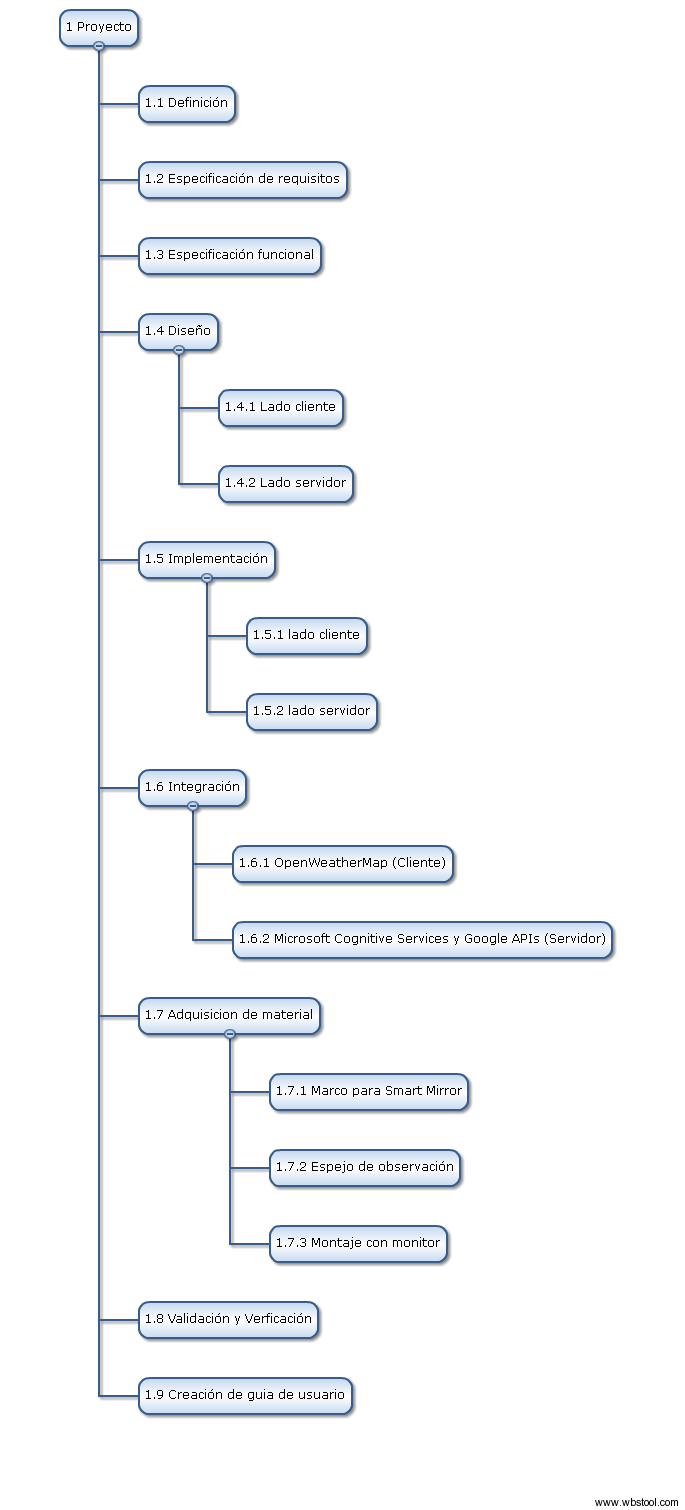
\includegraphics[angle=0, scale=.5]{fig/EDT}
	\caption{EDT}\label{fig:edt}
\end{figure}

Este desarrollo por etapas incluye las siguientes:

\begin{enumerate}
	\item \textbf{Plan operativo:}

	Etapa donde se define el problema a resolver, las metas del proyecto, las metas de calidad y se identifica cualquier restricción aplicable al proyecto.

	\item \textbf{Especificación de requisitos:}

	Permite entregar una visión de alto nivel sobre el proyecto, poniendo énfasis en la posibilidad de una planificación de los recursos sobre una escala de tiempos.

	\item \textbf{Especificación funcional:}

	Especifica la información sobre la cual el software trabajará.

	\item \textbf{Diseño:}

	Permite describir como el sistema va a satisfacer los requisitos.

	\item \textbf{Implementación:}

	Codificación del software.

	\item \textbf{Validación y verificación:}

	Etapa en la que se determina si el software desarrollado cumple con las especificaciones.
	
	\item \textbf{Mantenimiento:}

	Realización de arreglos y mejoras en el software desarrollado.

\end{enumerate}
\subsection{Productos intermedios}

Los productos intermedios que se generarán en cada una de las fases son:

\begin{itemize}
	\item Especificación de Requisitos

	\item Diseño del software

	\item Software funcional

	\item Hardware para Smart Mirror (un monitor encapsulado en un marco con espejo)

	\item Guía del usuario

\end{itemize}
\subsection{Tareas principales}

La implantación del proyecto comprende las siguientes tareas o actividades: 

\begin{itemize}

	\item \textbf{T1}	

	Definición del problema: En esta tarea se define el problema y se establecen una serie de ideas fundamentales para el proyecto, por ejemplo, el número de subsistemas por el que va a estar compuesta la solución. 
	\item \textbf{T2}	

	Especificación de requisitos: En esta tarea se deciden los requisitos funcionales y no funcionales que debe cumplir cada pieza de software a desarrollar en el proyecto.

	\item \textbf{T3}	

	Especificación funcional: En esta tarea se hace un diseño de alto nivel del software a implementar.

	\item \textbf{T4}

	Diseño del software: En esta tarea se detalla cómo se va a trabajar sobre las plantillas de software existente para crear un producto que satisfaga las especificaciones.

	\item \textbf{T4.1}

	Diseño del lado cliente.

	\item \textbf{T4.2}	

	Diseño del lado servidor.

	\item \textbf{T5}

	Implementación: En esta tarea se codifica todo lo diseñado en la tarea 4.
	
	\item \textbf{T5.1}
	
	Implementación de la funcionalidad base del cliente.
	
	\item \textbf{T5.2}
	
	Implementación de la funcionalidad base del servidor.
	
	\item \textbf{T6}
	
	Integración: En esta tarea se codifica todo lo necesario para que los múltiples sistemas incluidos en la solución trabajen juntos.
	
	\item \textbf{T6.1}
	
	Integrar cliente con servidor y API de OpenWeatherMap.
	
	\item \textbf{T6.2}	
	
	Integrar servidor con Microsoft Cognitive Services y Google APIs.
	
	\item \textbf{T7}	
	
	Adquisición de material para el Smart Mirror.
	
	\item \textbf{T7.1}	
	
	Adquisición de marco para Smart Mirror.
	
	\item \textbf{T7.2}
	
	Adquisición de espejo de observación.
	
	\item \textbf{T7.3}	
	
	Montaje con monitor.
	
	\item \textbf{T8}	
	
	Validar y verificar software.
	
	\item \textbf{T9}	
	
	Creación de guía de usuario.

\end{itemize}

\section{Organización y equipo}

\subsection{Esquema organizativo}

\begin{figure}[!htp]
	\centering
	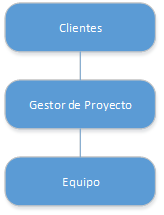
\includegraphics[scale=1.0]{fig/esquema_organizativo}
	\caption{Esquema organizativo}\label{fig:org_schema}
\end{figure}
\subsection{Plan de recursos humanos}\label{sec:planRecursosHumanos}

En el desarrollo del proyecto harán falta 3 tipos de recursos fundamentales, un gestor de proyecto, un consultor informático y un programador, los tres roles serán cubiertos por el Ingeniero Santiago Mazagatos Pérez.

\begin{itemize}
	\item \textbf{Gestor de proyecto:} 
	Su función es encargarse de la adquisición de todos los materiales necesarios para llevar a cabo el proyecto y asegurarse que las primeras etapas del proyecto se llevan a cabo respetando la visión y el objetivo final del mismo.
	\item \textbf{Consultor software:} 
	Su función es ayudar a enfocar el proyecto para diseñar un producto que no solo cumple con su función, sino que es fácil de usar por el usuario medio, también es el encargado de crear una pequeña guía de usuario.
	\item \textbf{Programador:} 
	Encargado de diseñar e implementar todo el software del producto.
\end{itemize}

\section{Condiciones de ejecución}

\subsection{Entorno de trabajo}

El lugar de trabajo habitual serán las instalaciones del equipo de trabajo.

El calendario y el horario serán propios del equipo de trabajo, trabajando 5 días a la semana, 8 horas al día excepto festivos según las festividades de la zona de Bilbao y nacionales. El día laboral empezará a las 8:00 de la mañana y terminará a las 17:00, con una hora de descanso de 13:00 a 14:00.

El equipo dependerá de sus propios medios para desarrollar y realizar los objetivos del proyecto, dichos medios se listan a continuación:


\begin{itemize}
	\item Ordenador personal
	\item Raspberry Pi 2 Model B 
	\item Webcam Logitech C210
	\item Servidor Microsoft Azure para desplegar servidor
	\item Servidor Microsoft Azure para albergar la \acrshort{bd} \acrshort{sql}
	\item Monitor de ordenador
	\item Marco con espejo de observación
	\item Software
	\begin{itemize}
		\item Microsoft Visual Studio Enterprise 2015
		\item Microsoft Windows 10 \acrshort{iot} Core
		\item Microsoft Office 2016
	\end{itemize}
\end{itemize}
\subsection{Control de cambios}

Cualquier cambio que se formule sobre especificaciones o productos ya realizados ha de ser revisado y aprobado por el equipo de desarrollo al completo para poderse realizar, siguiendo el siguiente procedimiento:

\begin{enumerate}
	\item Comunicación formal por parte del solicitante de las modificaciones requeridas.
	\item Valoración, por parte del Equipo de proyecto de la repercusión técnica, económica y del plazo de ejecución, en el caso de que acepten la modificación se pasa al siguiente paso, si no, el cambio no se realizará.
	\item Presentación de la propuesta de modificación al solicitante.
	\item Notificación por parte del solicitante de la aprobación o no de la propuesta.
	\item En caso afirmativo, modificación del plan de trabajo y del presupuesto.
\end{enumerate}
\subsection{Recepción de productos}

Los documentos tales como, diseños, especificaciones funcionales, documentación, análisis, controles, etc. que son la base de partida para trabajos posteriores deberán ser aprobados por el equipo de trabajo tras ser sometidos a escrutinio para ser mostrados a los clientes.

\section{Planificación}

En esta sección se exponen los diversos aspectos relacionados con la planificación del proyecto. Para facilitar la compresión de los datos y figuras que se van a mostrar más adelante, en la tabla \ref{tab:task_id_name}, se expone la relación entre los identificadores de las tareas y sus denominaciones.

\begin{table}[htp]
	\centering
	\caption{Relación identificador-tarea}\label{tab:task_id_name}
	\begin{tabular}{cc}
		\toprule
    	\textbf{Identificador} & \emph{Nombre}\\
    	\midrule
		T1 & Definición del problema\\
		T2 & Especificación de requisitos\\
		T3 & Especificación funcional\\
		T4 & Diseño del software\\
		T5 & Implementación\\
		T6 & Integración\\
		T7 & Adquisición de material para el Smart Mirror\\
		T8 & Validar y verificar software\\
		T9 & Creación de guía de usuario\\
    	\bottomrule
    \end{tabular}
\end{table}

\subsection{Diagrama de precedencias}

En esta sección se muestra el diagrama de precedencias (ver figura \ref{fig:network_diagram}).

\begin{figure}[!htbp]
	\centering
	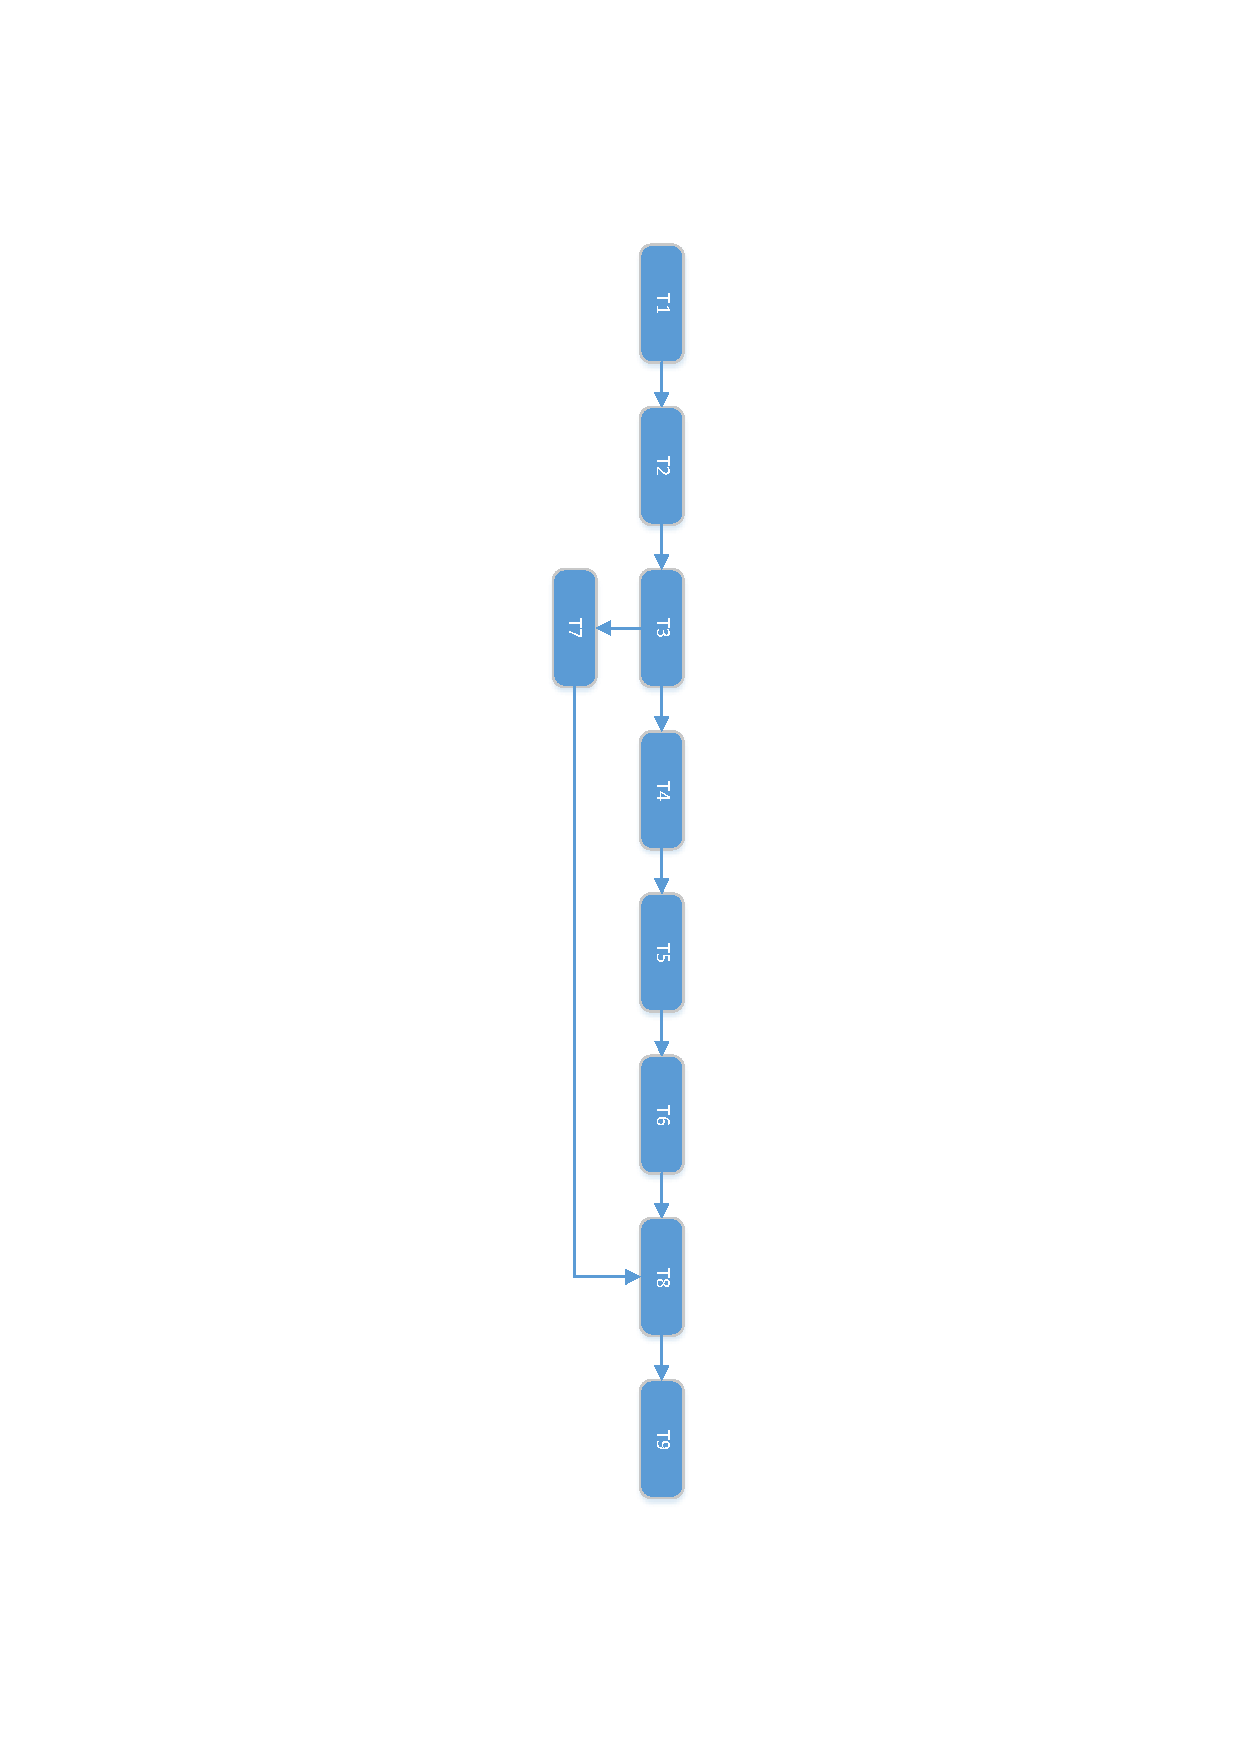
\includegraphics[page=1, scale=.8]{fig/diagrama_precedencias}
	\caption{Diagrama de precedencias}\label{fig:network_diagram}
\end{figure}

\FloatBarrier

\subsection{Plan de trabajo}

En la tabla \ref{tab:work_plan} se especifica el plan de trabajo planificado.

\begin{table}[htp]
	\centering
	\caption{Plan de trabajo}\label{tab:work_plan}
	\begin{tabular}{cccccc}
		\toprule
    	\textbf{Tarea} & \emph{Duración} & \emph{Trabajo} & \emph{Comienzo} & \emph{Fin} & \emph{Predecesoras}\\
    	\midrule
		T1	&	1 día		&	8 horas		&	lun 5/2/16	&	lun 5/2/16	&	-\\
		T2	&	2 días		&	16 horas	&	mar 5/3/16	&	mié 5/4/16	&	T1\\
		T3	&	2 días		&	16 horas	&	jue 5/5/16	&	vie 5/6/16	&	T2\\
		T4	&	4 días		&	32 horas	&	lun 5/9/16	&	jue 5/12/16	&	T3\\
		T5	&	10 días 	&	80 horas	&	vie 5/13/16	&	jue 5/26/16	&	T4\\
		T6	&	4 días		&	32 horas	&	vie 5/27/16 &	mié 6/1/16	&	T5\\
		T7	&	10 días		&	3 horas		&	jue 6/2/16	&	mié 6/15/16	&	T6\\
		T8	&	2 días		&	16 horas	&	jue 6/16/16	&	vie 6/17/16	&	T6;T7\\
		T9	&	1 día		&	8 horas		&	lun 6/20/16	&	lun 6/20/16	&	T8\\
    	\bottomrule
    \end{tabular}
\end{table}

\FloatBarrier

A continuación, en la tabla \ref{tab:recursos} se especifica los recursos, las horas de trabajo de y la proporción de la participación en cada una de las tareas.

\begin{table}[htp]
	\centering
	\caption{Recursos de las tareas}\label{tab:recursos}
	\begin{tabular}{cccc}
		\toprule
		\textbf{Tarea} & \emph{Recurso} & \emph{Horas}\\
		\midrule
	T1	&	Consultor informático	&	7 horas\\
	T1	&	Gestor de Proyecto		&	1 hora\\
	T2	&	Consultor informático	&	2 horas\\
	T2	&	Gestor de Proyecto		&	14 horas\\
	T3	&	Consultor informático	&	7 horas\\
	T3	&	Gestor de Proyecto		&	2 horas\\
	T3	&	Programador				&	7 horas\\
	T4	&	Programador				&	32 horas\\
	T5	&	Programador				&	80 horas\\
	T6	&	Programador				&	32 horas\\
	T7	&	Gestor de Proyecto		&	3 horas\\
	T8	&	Consultor informático	&	4 horas\\
	T8	&	Programador				& 	12 horas\\
	T9	&	Consultor informático	& 	8 horas\\

		\bottomrule
    \end{tabular}
\end{table}
\subsection{Diagrama de Gantt}

En esta sección se muestra el diagrama de Gantt (figura \ref{fig:gantt_diagram}).

\begin{figure}[!htp]
	\centering
	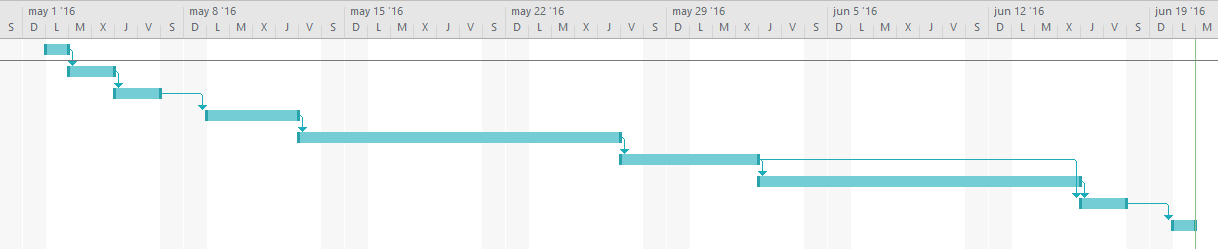
\includegraphics[angle=90, page=1, scale=.6]{fig/diagrama_gantt}
	\caption{Diagrama de Gantt}\label{fig:gantt_diagram}
\end{figure}


\FloatBarrier

\subsection{Estimación de cargas de trabajo por perfil}

En esta sección se muestra la estimación de cargas de trabajo separado por los perfiles que existen en el proyecto (vease la tabla \ref{tab:workload})

\begin{table}[htp]
	\centering
	\caption{Cargas de trabajo por perfil}\label{tab:workload}
	\begin{tabular}{cc}
		\toprule
    	\textbf{Perfil de trabajo} & \emph{Carga de trabajo(h)}\\
    	\midrule
		Consultor informático	&	28 horas\\
		Gestor de Proyecto		&	20 horas\\
		Programador				&	163 horas\\
    	\bottomrule
    \end{tabular}
\end{table}

\section{Presupuesto}

En esta sección se detalla el presupuesto planificado para la realización de proyecto. El presupuesto se desglosa en tres apartados diferentes: Recursos Humanos, Software y Hardware.

\subsection{Recursos humanos}

En la tabla \ref{tab:budget-human} se detalla los honorarios por cada uno de los roles, dependiendo de las horas que trabaja según lo planificado.

\begin{table}[htp]
	\centering
	\caption{Presupuesto de recursos humanos}\label{tab:budget-human}
	\begin{tabular}{cccc}
		\toprule
    	\textbf{Rol} & \emph{Precio/hora(\euro/h)} & \emph{Carga de trabajo(h)} & \emph{Importe total(\euro)}\\
    	\midrule
		Consultor informático	&	40.64€/hora	&	28 horas	&	1,137.92€\\
		Gestor de Proyecto		&	55.46€/hora	&	20 horas	&	1,109.20€\\
		Programador				&	38.24€/hora	&	163 horas	&	6,233.12€\\
    	\bottomrule
    \end{tabular}
\end{table}
\subsection{Recursos software}

En la tabla \ref{tab:budget-software} se detalla el gasto destinado a las herramientas software según lo planificado.

\begin{table}[htp]
	\centering
	\caption{Presupuesto de software}\label{tab:budget-software}
	\begin{tabular}{cccc}
		\toprule
    	\textbf{Nombre} & \emph{Importe total(\euro)}\\
    	\midrule
		Microsoft Office 2016					&	99.00€\\
		Microsoft Visual Studio Enterprise 2015	&	500.00€\\
    	\bottomrule
    \end{tabular}
\end{table}
\subsection{Recursos hardware}

En la tabla \ref{tab:budget-hardware} se detalla el gasto destinado a los dispositivos hardware según planificado.

\begin{table}[htp]
	\centering
	\caption{Presupuesto de hardware}\label{tab:budget-hardware}
	\begin{tabular}{cccc}
		\toprule
    	\textbf{Nombre} & \emph{Precio(\euro)}\\
    	\midrule
		Raspberry Pi 2 Model B	&	55.00€\\
		Monitor Acer H243HQ		&	200.00€\\
		Marco para Smart Mirror	&	60.00€\\
		Espejo de observación	&	110.00€\\
		Webcam Logitech C210	& 	30.00€\\
    	\bottomrule
    \end{tabular}
\end{table}
\subsection{Total}

Para finalizar, en la tabla \ref{tab:total-budget} se detalla el presupuesto total, que se calcula mediante la suma del costo estimado de los Recursos Humanos, el Software y el Hardware.

\begin{table}[htp]
	\centering
	\caption{Presupuesto total}\label{tab:total-budget}
	\begin{tabular}{cc}
		\toprule
    	\textbf{Tipo} 		& 	\emph{Total}\\
    	\midrule
		Recursos humanos	&	8,480.24€\\
		Recursos software	&	599.00€\\
		Recursos hardware	&	455.00€\\
		\textbf{Total}		&	\textbf{9,534.24€}\\
    	\bottomrule
    \end{tabular}
\end{table}
\chapter{Especificación de requisitos}

\section{Visión general}

En el capítulo de especificación de requisitos se detallan los requisitos que deben cumplir cada uno de los componentes del sistema con el fin de que todo funcione correctamente, tanto el cliente como el servidor tienen una sección dedicada a sus requisitos.

\begin{itemize}
	\item \textbf{Especificación de requisitos del cliente \acrshort{uwp}:} en esta sección se recogen los requisitos que debe de satisfacer el cliente que actuará como Smart Mirror.

	\item \textbf{Especificación de requisitos del servidor:} en esta sección se recogen los requisitos que debe satisfacer el servidor encargado de proporcionarle informacion y servicios al Smart Mirror.
\end{itemize}

\section{Especificación de requisitos del cliente \acrshort{uwp}}

Los requisitos del cliente \acrshort{uwp} son:

\begin{itemize}
	\item \textbf{RF.0.1}

	El cliente debe ser capaz de usar una webcam para sacar fotos de forma periódica.

	\item \textbf{RF.0.2}

	El cliente debe ser capaz de determinar su posición geográfica mediante su conexión a internet.

	\item \textbf{RF.0.3}

	El cliente debe ser capaz de realizar peticiones correctas a la API de OpenWeatherMap y parsear las respuestas.

	\item \textbf{RF.0.4}

	El cliente debe ser capaz de enviar las imágenes que captura al servidor de forma correcta y parsear las respuestas del mismo.

	\item \textbf{RNF.0.1}

	La información debe ser presentada al usuario de forma elegante y clara.

\end{itemize}


\section{Especificación de requisitos del servidor}

Los requisitos del servidor son los siguientes:

\begin{itemize}
	\item \textbf{RF.0.1}

	El servidor debe ser capaz de recibir imágenes del cliente y almacenarlas para su uso para funciones de identificación.

	\item \textbf{RF.0.2}

	El servidor debe ser capaz de autenticar a los usuarios por medio de Google y de almacenar datos adicionales como una URL correspondiente a una foto del usuario, proporcionada por este.

	\item \textbf{RF.0.3}

	El servidor debe ser capaz de extraer información de los perfiles de Google de los usuarios, en concreto eventos de calendario, tareas y mensajes de correo electrónico.

	\item \textbf{RF.0.4}

	El servidor debe ser capaz de usar la API de Microsoft Cognitive Services para comparar imágenes e identificar usuarios.

	\item \textbf{RNF.0.1}
	
	El proceso de registro debe ser simple y rápido para el usuario.
	
\end{itemize}

\section{Criterios de validación}

El cumplimiento de los requisitos por parte de los productos software se garantizan mediante pequeños tests unitarios que comprueban la funcionalidad del software con datos de prueba antes de integrarlo con el resto del sistema.
\chapter{Tecnologías utilizadas}

\section{Visión general}

En esta sección se presentan las diferentes tecnologías que se han utilizado para el desarrollo del proyecto. Las principales tecnologías usado son las siguientes:

\section{Microsoft Azure}

Microsoft Azure\cite{Azure} es una plataforma e infraestructura de cloud computing creada por Microsoft para desarrollar, desplegar y gestionar aplicaciones y servicios a través de una red global de data centers gestionados por Microsoft.
Proporciona servicios tanto \acrshort{paas} como \acrshort{iaas} y soporta una multitud de lenguajes de programación, herramientas e infraestructuras, ya sean propias de Microsoft o de terceros.

\begin{figure}[!htbp]
	\centering
	
\includegraphics[scale=1.2]{fig/microsoft_azure}
	\caption{Logotipo de Microsoft Azure}
\end{figure}

Los servicios de Azure utilizados en este proyecto son los siguientes:
\begin{itemize}
	\item Creación y hospedaje de una aplicación web
	\item Creación y hospedaje de un servidor \acrshort{sql}
	\item Creación y hospedaje de una \acrshort{bd} \acrshort{sql}
\end{itemize}

\subsection{Razón de uso}

\begin{itemize}
	\item Al ser ambos productos de Microsoft, la integración entre Microsoft Azure y Microsoft Visual Studio Enterpise 2015 es inmejorable, haciendo que el despliegue de aplicaciones sea fácil y rápido.
	\item Familiaridad del equipo con la plataforma.
	\item Al ser un servicio ofrecido por un gigante de las tecnologías de información como Microsoft, se puede esperar que el servicio será seguro y fiable y cuente con un buen soporte en el caso de incidencias.

\end{itemize}

\section{Microsoft Cognitive Services}

Microsoft Cognitive Services\cite{Oxford} (anteriormente Project Oxford) es un conjunto de \acrshort{api}s, \acrshort{sdk}s y servicios disponibles a los desarrolladores para que hagan sus aplicaciones más inteligentes, interactivas y accesibles. Microsoft Cognitive Services expande el abanico ya existente de APIs de machine learning creadas por Microsoft y permite a los desarrolladores añadir características inteligentes de forma fácil, tales como reconocimiento de voz, facial, emoción y visión, así como comprensión de lenguaje natural.

\subsection{Razón de uso}

\begin{itemize}
	\item Existencia de pruebas gratuitas
	\item Documentación extensa, clara y concisa.

\end{itemize}

\section{Universal Windows Platform}

La \acrfull{uwp}\cite{UWP} es una arquitectura de aplicación homogénea creada por Microsoft y introducida por primera vez en Windows 10, el propósito de esta plataforma es ayudar a desarrollar aplicaciones de estilo Metro que puedan ejecutarse en cualquier dispositivo Windows 10 sin necesidad de ser reescritas, soporta el desarrollo de aplicaciones de Windows usando C++, C\#, \acrshort{vb.net} o \acrshort{xaml}. La API está implementada en C++ y soportada en C++, \acrshort{vb.net}, C\#, F\# y \acrfull{js}. Diseñada como una extensión de la plataforma Windows Runtime introducida en Windows Server 2012 y Windows 8, \acrshort{uwp} permite a los desarrolladores crear aplicaciones que puedan, potencialmente, ejecutarse en múltiples tipos de dispositivos.

\begin{figure}[!htbp]
	\centering
	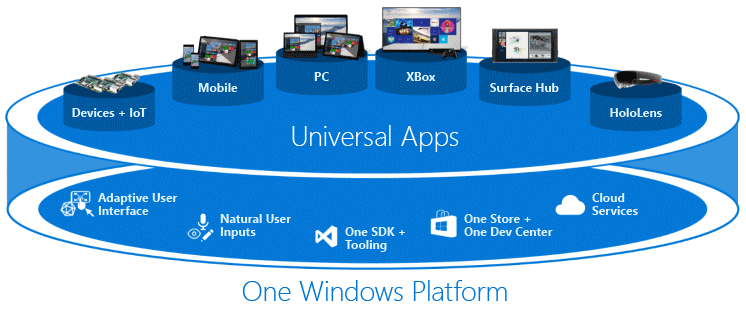
\includegraphics[scale=0.7]{fig/uwp_representation}
	\caption{Representación de \acrshort{uwp}}
\end{figure}

\FloatBarrier

\subsection{Razón de uso}

La Plataforma Universal Windows proporciona recursos como Windows.Media.Capture o Windows.Devices.Geolocation, que son utilizados en este proyecto, \acrshort{uwp} incluye muchas librerías que permiten a un programador acceder a los recursos del sistema de una forma estandarizada sin necesidad de preocuparse de que hardware se use, con MediaCapture, una aplicación \acrshort{uwp} es capaz de usar el mismo código para acceder a una cámara \acrshort{usb} de hace 10 años y una que acaba de salir de la fábrica, siempre y cuando el sistema tenga los drivers adecuados, se da el mismo caso con la librería Geolocation, no siendo necesario hacer ninguna consideración sobre que hardware debe tener el dispositivo, independientemente de si el dispositivo en el que el código se ejecuta tenga \acrshort{gps}, \acrshort{wifi} o una conexión por cable a internet, el código subyacente determinará la posición del dispositivo de la manera que estime conveniente de acuerdo con la petición que se le ha realizado (si se requiere alta precisión, o no), esto hace que la codificación de funciones complejas que hace años habría llevado una gran cantidad de tiempo hoy en día se pueda hacer en menos de una hora.

\lstinputlisting[frame=single, caption=Código para manejo de WebCam]{content/code/mediacapture.cs}
\lstinputlisting[frame=single, caption=como obtener la localización del dispositivo]{content/code/geolocation.cs}

\section{ASP.NET}

ASP.NET\cite{asp.net} es una infraestructura open-source de aplicaciones web server-side diseñada para el desarrollo web de páginas web dinámicas, fue originalmente desarrollada exclusivamente por Microsoft, es ideal para crear paginas basadas en los estándares \acrshort{html}5, \acrshort{css}3 y \acrfull{js} e incluye tres maneras distintas de trabajar:

\begin{itemize}

\item \textbf{ASP.NET Web Forms:} usa controles y un modelo de eventos para un desarrollo basado en componentes

\item \textbf{ASP.NET \acrshort{mvc}:} \acrshort{mvc} valora la separacion de conceptos y permite usar la metodología \acrshort{tdd} de una forma mas facil

\item \textbf{ASP.NET Web Pages:} Web Pages prefiere un modelo de página unica que mezcla codigo y marcado \acrshort{html}.

\end{itemize}

Todas estas técnicas se pueden mezclar en la misma aplicación al ser todo ASP.NET

\begin{figure}[!htbp]
	\centering
	
\includegraphics[scale=0.6]{fig/asp-net_highlights}
	\caption{Aspectos destacados de ASP.NET}
\end{figure}

ASP.NET incluye la ASP.NET Web \acrshort{api} para crear servicios \acrshort{rest}-ful de calidad que devuelvan \acrshort{json}, \acrshort{xml} o cualquier tipo de contenido que soporte la web, las ASP.NET Web \acrshort{api}s pueden proveer servicios de datos a aplicaciones móviles como las de Windows Phone, iPhone, Android y más, también pueden ser usadas en cualquier tipo de aplicación ASP.NET, ya sea Web Forms, \acrshort{mvc} o Web Pages.

ASP.NET SignalR es una librería para desarrolladores de ASP.NET que convierten la comunicación bi-direccional de cliente y servidor en tiempo real en realidad, SignalR permite el uso de nuevos estándares como Web Sockets manteniendo la compatibilidad con exploradores más antiguos, puede soportar clientes \acrfull{js}, al igual que clientes en Android, iPhones y todos los clientes basados en C# como Windows Phone y Windows 8.

ASP.NET puede usarse para crear aplicaciones móviles con \acrshort{rwd} gracias a tener Twitter Bootstrap incorporado desde Visual Studio 2013, se puede usar cualquier framework \acrshort{css} o sistemas como JQuery Mobile o Sencha.

Stack Overflow\cite{StackOverflow} usa ASP.NET \acrshort{mvc} para su página junto a \acrshort{sql} Server y otras tecnologías de Microsoft

En este caso en concreto se ha utilizado ASP.NET \acrshort{mvc}, radicalmente distinto a ASP.NET Web Forms y que usa el patrón \acrfull{mvc}.

\begin{figure}[!htbp]
	\centering
	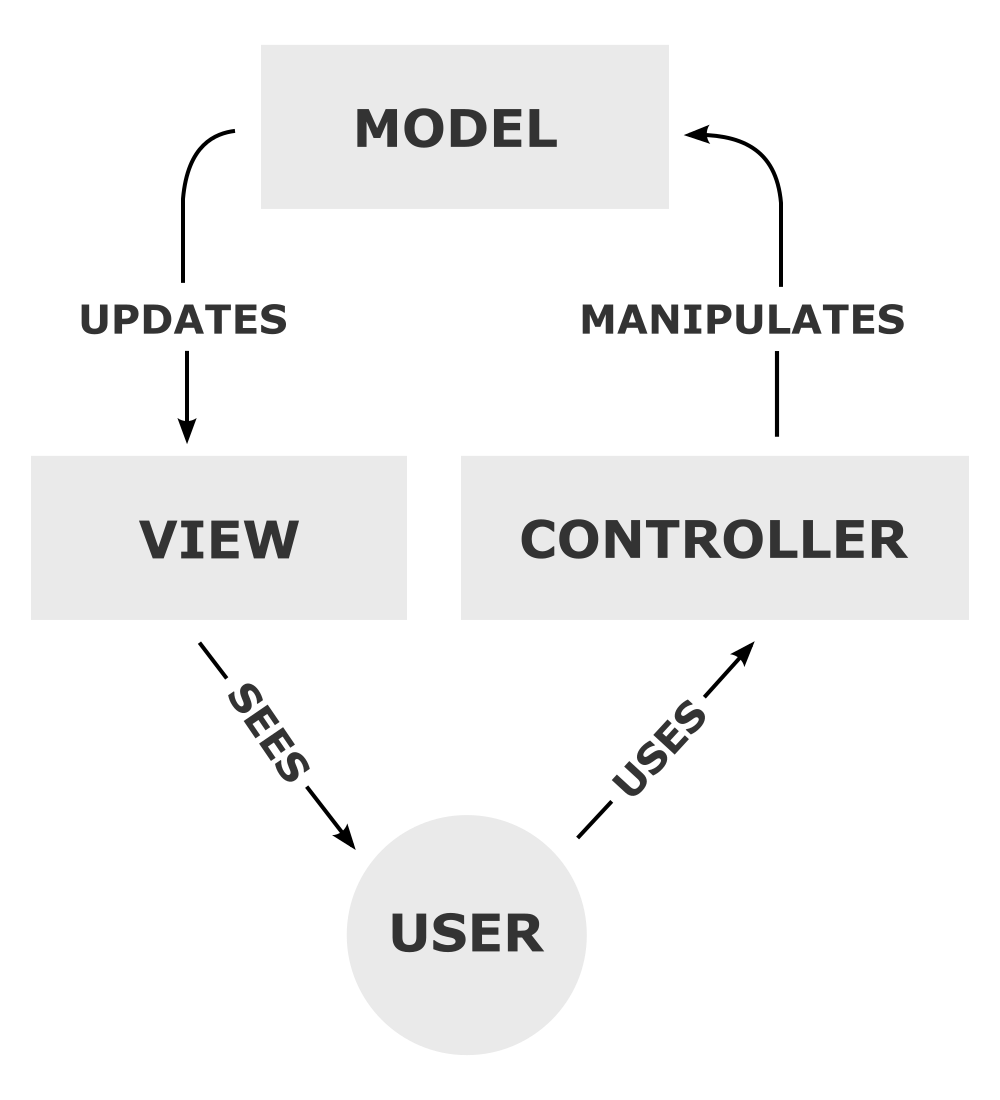
\includegraphics[scale=0.50]{fig/mvc_pattern}
	\caption{Representación del patrón \acrshort{mvc}}
\end{figure}

\subsection{ASP.NET Razor}

Razor es una sintaxis de programación de ASP.NET usada para crear páginas web dinámicas con \acrshort{vb.net} o C#, Razor fue lanzado para Visual Studio 2010 en enero de 2011 como parte de ASP.NET \acrshort{mvc} 3 y el set de herramientas WebMatrix.

\lstinputlisting[frame=single, caption=Ejemplo de una vista en ASP.NET Razor]{content/code/externalloginview.cshtml}

\subsection{Razón de uso}

\begin{itemize}
	\item Una gran variedad de plantillas de calidad para desarrollar aplicaciones web rápidamente, así como placeholders para autenticación con servicios externos ya incluidos en ellas.
	\item Extensa documentación y tutoriales creados por Microsoft.
	\item Bootstrap integrado junto con la mayoría de las plantillas.

\end{itemize}

\section{Application Insights}

\acrfull{ai}\cite{AI}, también denominado Visual Studio \acrfull{ai} es una herramienta de depuración de errores que permite detectar y diagnosticar errores en una aplicación web sin tener que conectar un debugger a la misma.

\begin{figure}[!htbp]
	\centering
	
\includegraphics[scale=0.50]{fig/applicationinsights_logo}
	\caption{Logotipo de \acrfull{ai}}
\end{figure}

Usado por clientes como Xerox\cite{Xerox}, \acrshort{ai} permite realizar un amplio análisis de una página o aplicación web en ejecución, pudiendo recabar datos sobre fallos del servidor (excepciones, peticiones fallidas, etc.) o rendimiento (tiempo de respuesta, número de peticiones), \acrshort{ai} utiliza Machine Learning para analizar constantemente una aplicación y determinar su funcionamiento normal, para así detectar comportamientos anómalos de manera más efectiva, permitiendo a los desarrolladores encontrar errores en su aplicación antes de que estos afecten el funcionamiento del código de forma significativa.

\subsection{Razón de uso}

Al no poder estar monitorizando el servidor desplegado en Azure para servir de fuente de datos al Smart Mirror todo el rato mediante la conexión de un debugger de Visual Studio a este, \acrshort{ai} ha sido una herramienta inestimable para diagnosticar problemas que no son evidentes en una primera ejecución del código y que solo aparecen bajo circunstancias especiales.

\section{Bootstrap}

Boostrap\cite{Bootstrap} es una infraestructura gratuita y de código abierto para uso en front-ends de sitios y aplicaciones web, contiene plantillas basadas en \acrshort{html} y \acrshort{css} para tipografías, formularios, botones, elementos de navegación y otros componentes de interfaz, además de extensiones \acrfull{js} opcionales, a diferencia de muchos otros frameworks, se limita únicamente al desarrollo de front-ends.

\begin{figure}[!htbp]
	\centering
	
\includegraphics[scale=0.50]{fig/bootstrap_logo}
	\caption{Logotipo de Bootstrap}
\end{figure}

Bootstrap, originalmente llamado Twitter Blueprint fue desarrollado por Mark Otto y Jacob Thornton en Twitter como una infraestructura para fomentar la consistencia entre varias herramientas internas. Antes de Bootstrap, el desarrollo de interfaces se realizaba haciendo uso de varias librerías, lo cual causaba inconsistencias y representaba un gran obstáculo para el mantenimiento.

\subsection{Razón de uso}

Aparte de estar incluido en las plantillas de ASP.NET, Bootstrap proporciona una manera fácil y rápida de diseñar e implementar páginas que usen \acrfull{rwd}, y que tengan un aspecto agradable para el usuario, aparte de una gran cantidad de código \acrfull{js} para asegurarse de que la interfaz es lo más fluida posible.
\chapter{Especificación del diseño}\label{chap:design}

\section{Visión general}

Este capítulo tiene como objetivo describir la labor de diseño realizada para desarrollar el proyecto, así como las herramientas que han sido necesarias para su realización. En el siguiente listado se describen los aspectos de diseño que se van a explicar en este capítulo:

\begin{itemize}
	\item \textbf{Diseño de la aplicación cliente}: descripción de las modificaciones realizadas sobre una plantilla \acrshort{uwp}.
	\item \textbf{Diseño de la aplicación web}: descripcion de las modificaciones realizadas sobre una plantilla ASP.NET \acrshort{mvc}.

\end{itemize}

\section{Diseño de la aplicación cliente}

La Aplicación cliente cuenta con dos clases especiales para ocuparse de la lógica de las peticiones HTTP y de la lógica de uso de una cámara web.

\begin{figure}[!htbp]
	\centering
	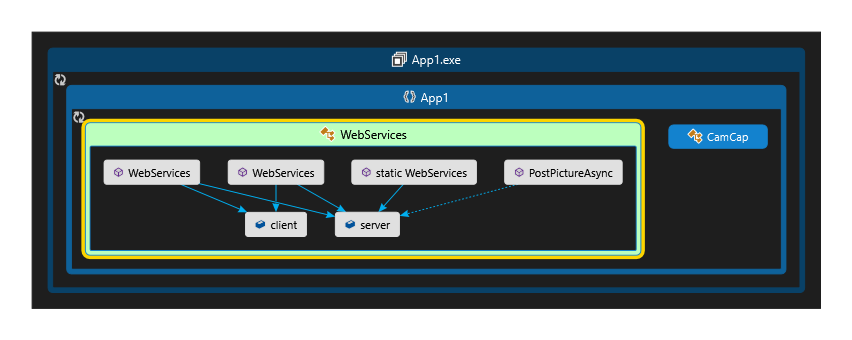
\includegraphics[angle=90, scale=1.0]{fig/WebServices}
	\caption{Clase WebServices}
\end{figure}

\FloatBarrier

\lstinputlisting[frame=single, caption=Clase WebServices]{content/code/webservices.cs}

\begin{figure}[!htbp]
	\centering
	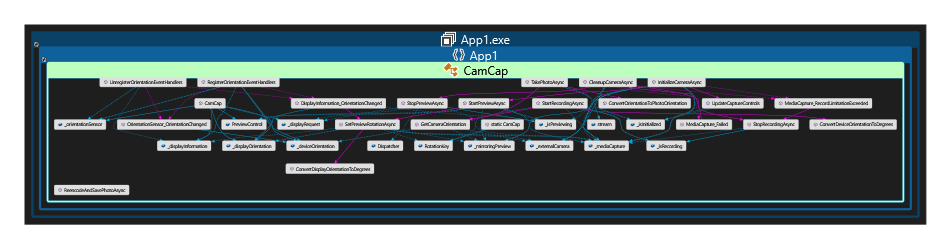
\includegraphics[angle=90, scale=0.9]{fig/CamCap}
	\caption{Clase CamCap}
\end{figure}

\FloatBarrier

Ya que la clase CamCap es en su mayoría parte de un ejemplo de Microsoft sobre el manejo correcto de una WebCam mediante la librería MediaCapture y no un código creado expresamente con el solo fin de capturar imágenes, la mayoría de los métodos, propiedades y variables del diagrama no se usan, aquí se incluyen las partes del código que se usan en el proyecto:

\begin{itemize}

\item \textbf{InitializeCameraAsync:} inicialización de la cámara.

\lstinputlisting[frame=single, caption=Código de InitializeCameraAsync]{content/code/initializecamera.cs}

\item \textbf{StartPreviewAsync:} acceso a una vista previa de lo que será capturado por la cámara.

\lstinputlisting[frame=single, caption=Código de StartPreviewAsync]{content/code/startpreview.cs}

\item \textbf{TakePhotoAsync:} se captura una imagen y se codifica en un stream.

\lstinputlisting[frame=single, caption=Código de TakePhotoAsync]{content/code/takephoto.cs}

\end{itemize}

\section{Diseño de la aplicación web}

La principal inclusión en la plantilla de la aplicación Web es un controlador para abordar todas las funciones necesarias.

\begin{figure}[!htbp]
	\centering
	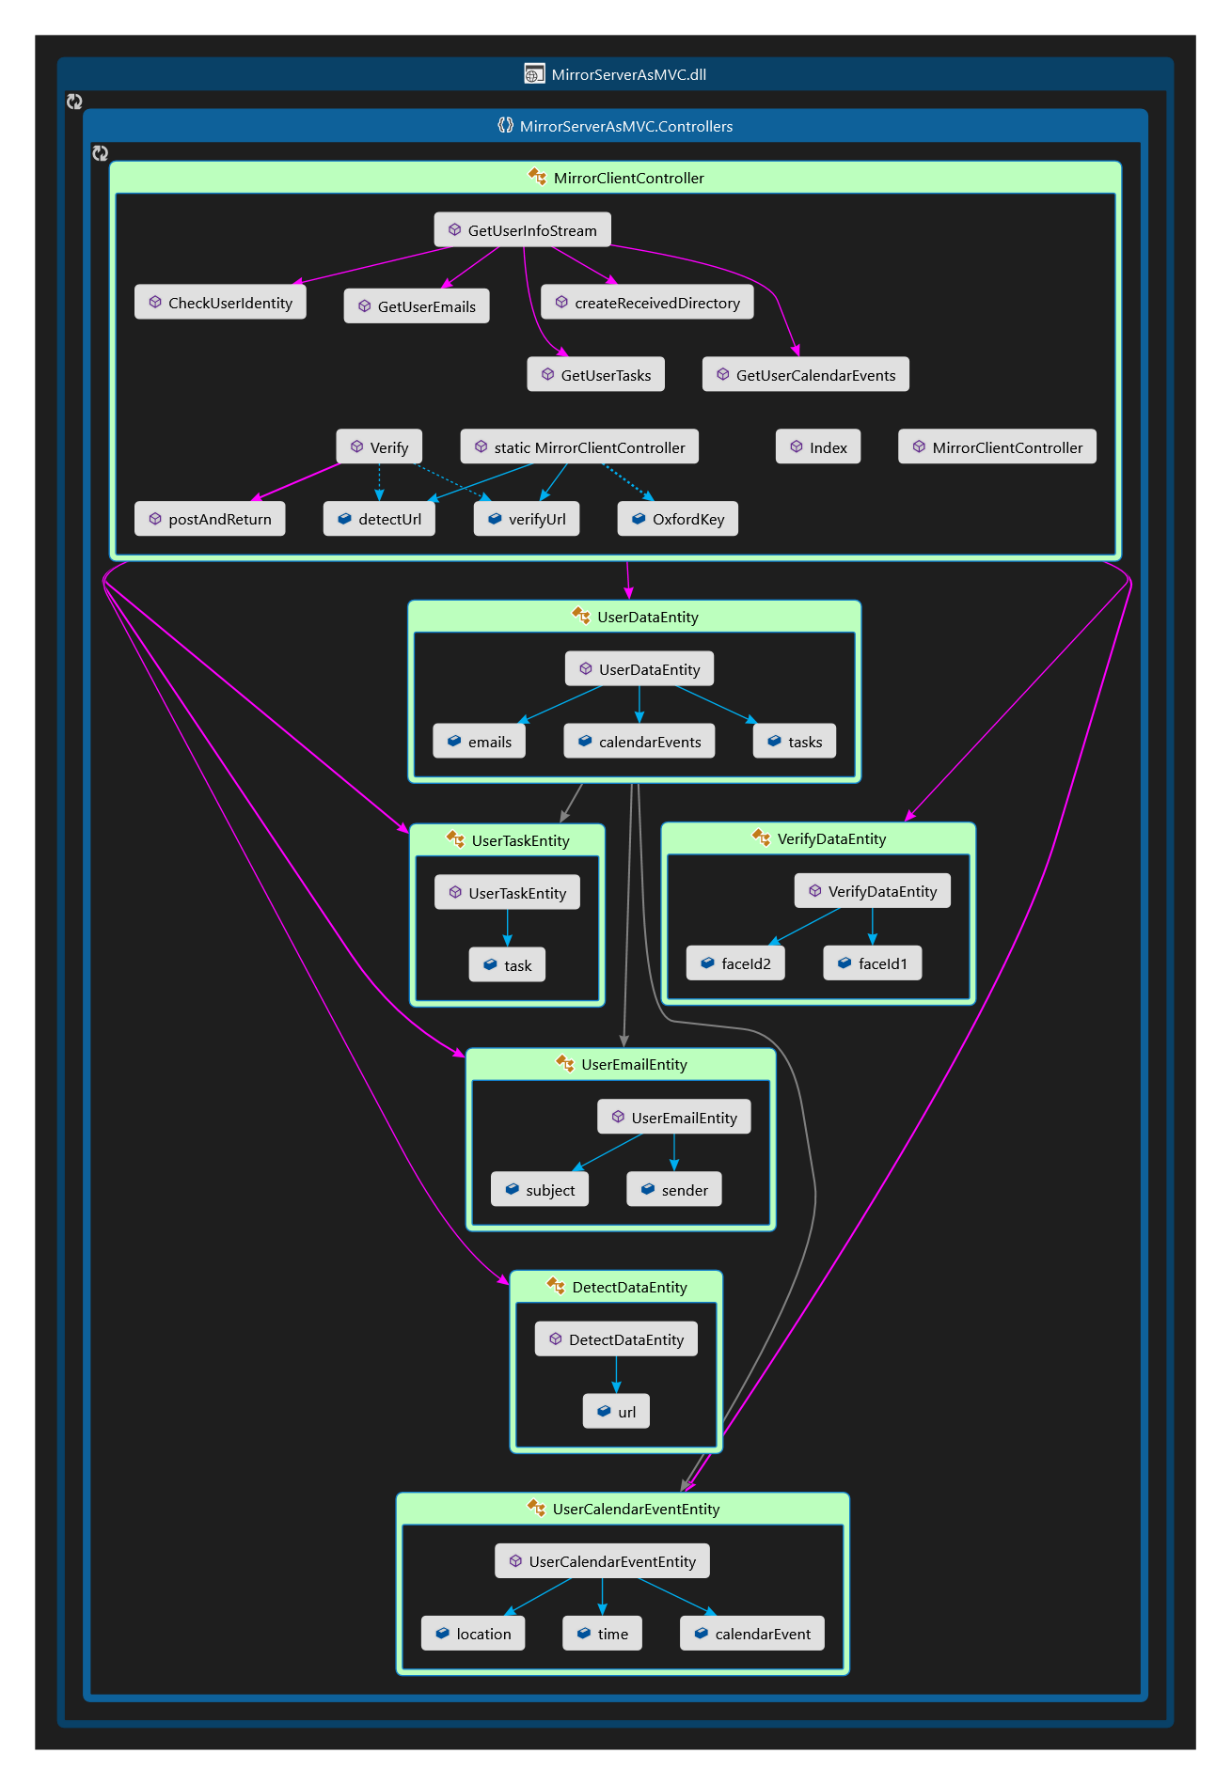
\includegraphics[angle=0, scale=1.0]{fig/MirrorClientController}
	\caption{Clase MirrorClientController}
\end{figure}

\FloatBarrier

A continuación se muestra el código que usa el servidor para recibir una imagen, almacenarla y usarla para verificar un usuario.

\lstinputlisting[frame=single, caption=Fragmento de código de MirrorClientController]{content/code/controller.cs}

\subsection{Modificación de la \acrshort{bd}}

Una aplicación ASP.NET \acrshort{mvc} configurada con autenticación crea por defecto una \acrshort{bd} con todas las tablas necesarias para autenticar usuarios y usar roles, en el caso de este proyecto se modificó el esquema para incluir tres campos en la tabla del usuario:

\begin{itemize}
\item \textbf{FaceId:} un id de cara proporcionado por Microsoft Cognitive Services, que expira a las 24 horas de ser generado.
\item \textbf{LastUpdate:} fecha en la que se actualizó el identificador de cara por ultima vez para comprobar si está expirado o no.
\item \textbf{PhotoUrl:} \acrshort{url} a una imagen del usuario para obtener nuevos FaceId y contrastarlos con los de las fotos que se reciban desde el Smart Mirror.
\end{itemize}

\begin{figure}[!htp]
	\centering
	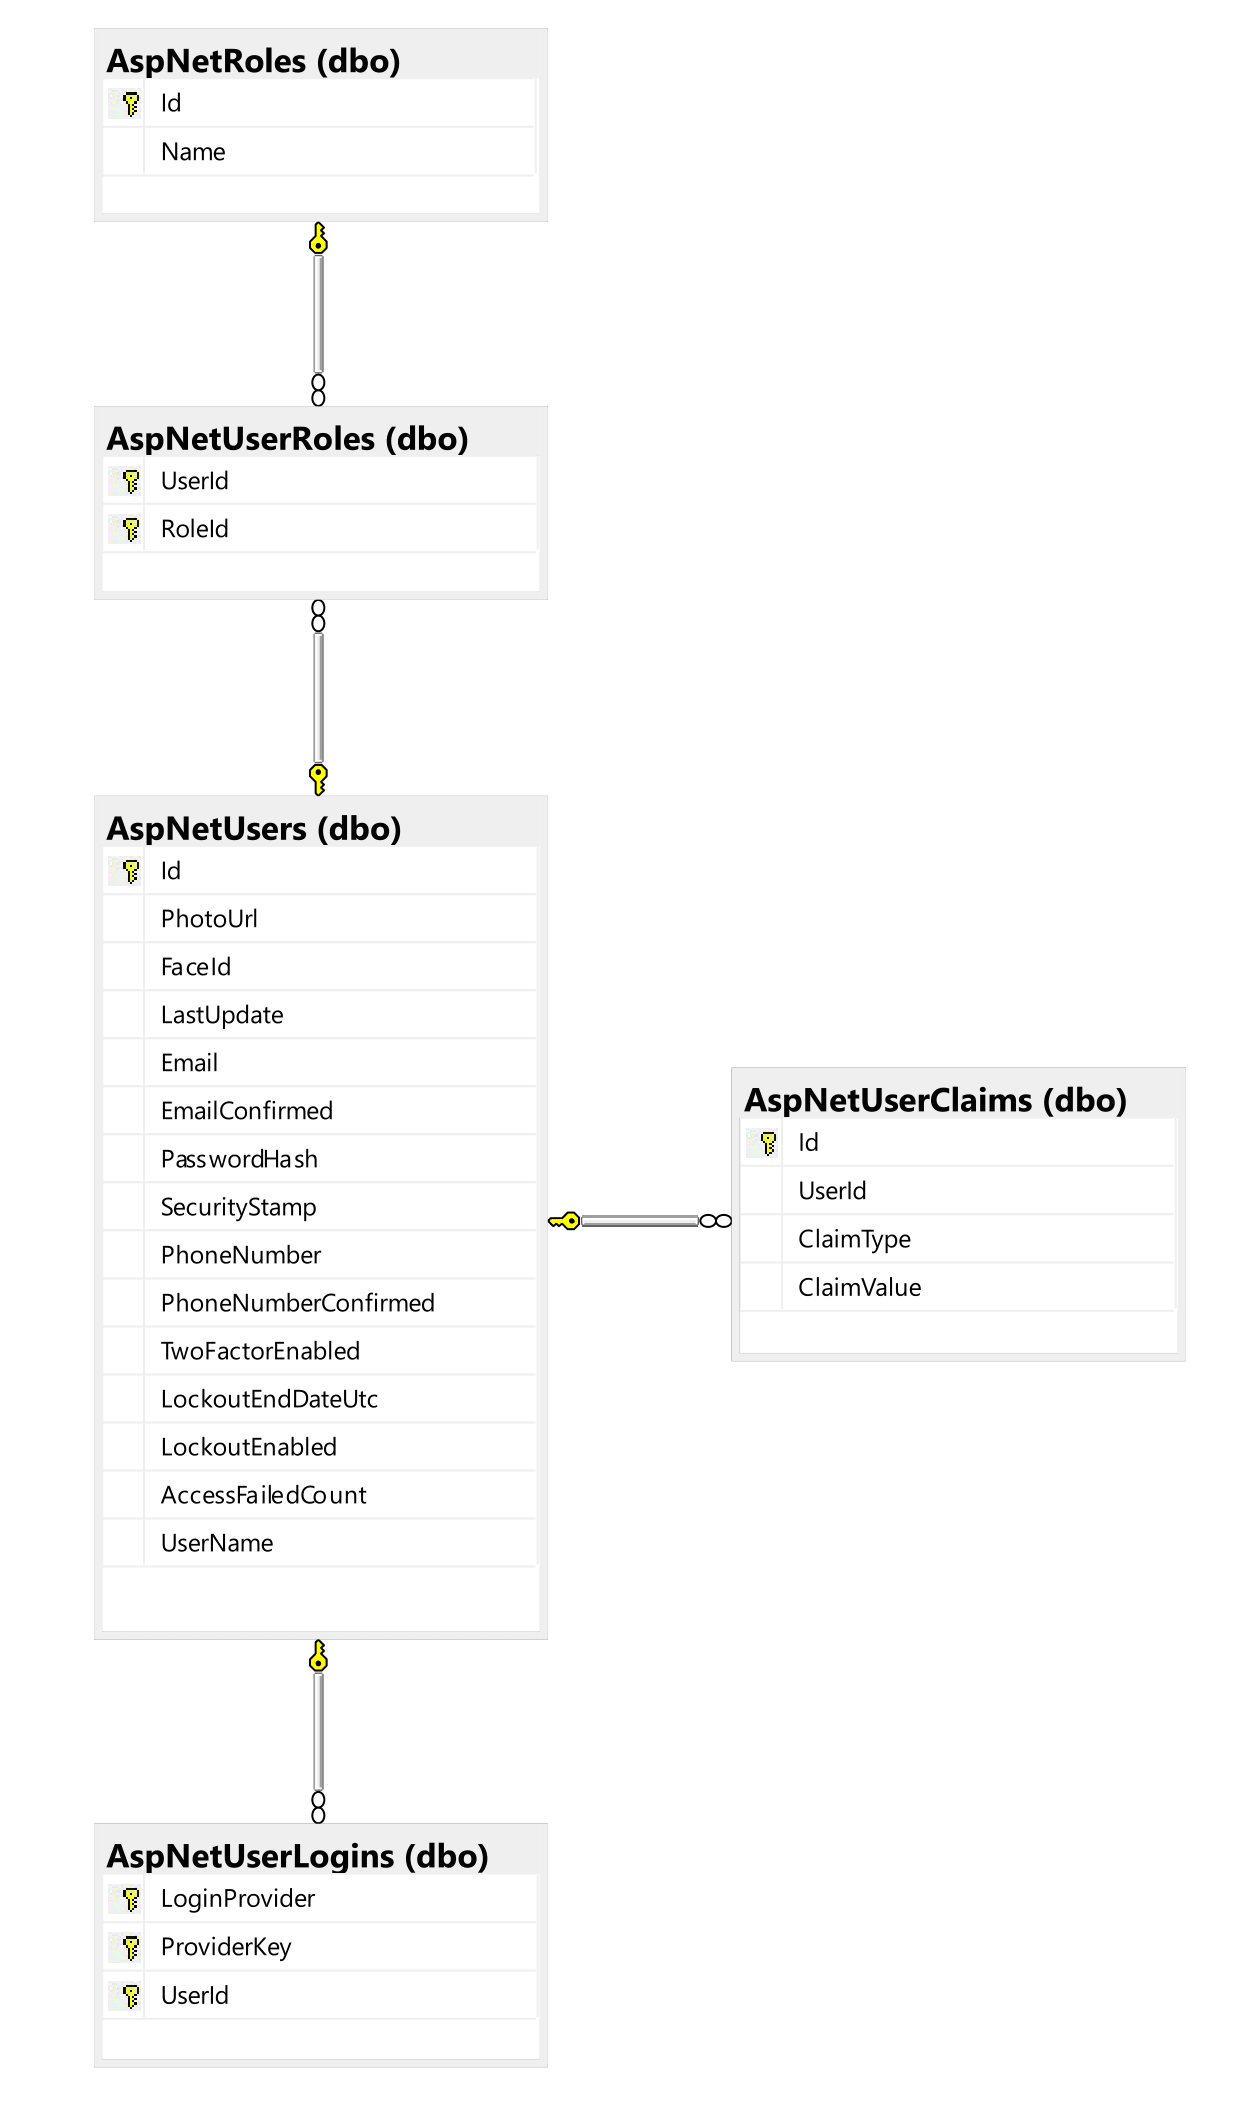
\includegraphics[angle=0, page=1, scale=.3]{fig/schema}
	\caption{Schema de la \acrshort{bd} modificada}
\end{figure}

\FloatBarrier

\chapter{Consideraciones sobre la implementación}

\section{Visión general}

Este capítulo detalla los aspectos más importantes a tener en cuenta para codificar el software.

\section{Entorno de desarrollo}

Estas son las herramientas utilizadas para la realización de este proyecto.

\subsection{Visual Studio}

Microsoft Visual Studio\cite{VisualStudio} es un entorno de desarrollo integrado creado por Microsoft, se usa para desarrollar programas para Microsoft Windows , así como páginas, aplicaciones y servicios web. Visual Studio usa plataformas de desarrollo de software como Windows \acrshort{api}, Windows Forms, Windows Presentation Foundation, Windows Store y Microsoft Silverlight. Puede producir tanto código nativo como gestionado.

\begin{figure}[!htp]
	 \centering
	 
\includegraphics[scale=1.0]{fig/visualstudio_logo}
	 \caption{Logotipo de Visual Studio}
\end{figure}

Visual Studio incluye un editor de código que soporta IntelliSense y refactorización de código. El debugger integrado funciona como un debugger a nivel de código fuente y a nivel de código máquina. Otras herramientas integradas que incluye Visual Studio son diseñadores para web, clases y esquemas de \acrshort{bd}. Acepta plug-ins que extienden la funcionalidad a casi cualquier nivel, incluido soporte añadido para sistemas de control de fuente como Subversion o la adición de sets de herramientas como editores y diseñadores visuales para lenguajes específicos de dominio o para otros aspectos del ciclo de desarrollo de software.

Visual Studio soporta varios lenguajes de programación y permite al editor y debugger soportar casi cualquier lenguaje de programación, siempre y cuando exista un servicio específico de ese lenguaje, los lenguajes integrados por defecto en Visual Studio incluyen C, C++ y \acrshort{cppcli}, VB.NET, C\# y F\#. Soporte para otros lenguajes como Python, Ruby, Node.js y M entre otros está disponible mediante servicios de lenguaje a instalar por separado, también soporta \acrshort{xml}/\acrshort{xslt}, \acrshort{html}/\acrshort{xhtml}, \acrfull{js} y \acrshort{css}. Java (y J\#) fueron soportados en el pasado.


\subsection{Google Chrome}

Google Chrome\cite{Chrome} es un explorador web gratuito desarrollado por Google. Usaba el WebKit layout engine hasta la versión 27 y con la excepción de sus versiones de iOS, desde la versión 28, Chrome usa Blink, fue en un principio lanzado como una versión beta para Microsoft Windows el 2 de septiembre de 2008 y finalmente como una versión estable el 11 de diciembre de 2008.

\begin{figure}[!htp]
	 \centering
	 
\includegraphics[scale=0.3]{fig/googleChrome_logo}
	 \caption{Logotipo de Google Chrome}
\end{figure}

A fecha de marzo de 2016, StatCounter estima que Google Chrome tiene un 60.1\% del mercado de los navegadores web como navegador de sobremesa, es también el navegador más usado en smartphones, su éxito ha dado lugar a que Google expanda la marca “Chrome” a otros productos como el Chromecast o Chromebook.

\subsection{Git}

Git\cite{Git} es un sistema de control de versión y es ampliamente utilizado en el ámbito del desarrollo de software y otras tareas de control de versión. Es un sistema distribuido con el énfasis puesto en su velocidad, integridad de datos y el soporte para flujos de trabajo distribuidos y no lineales. Git fue creado por Linus Torvalds en 2005 para el desarrollo del kernel Linux, con la colaboración de otros desarrolladores del kernel para su desarrollo inicial.

\begin{figure}[!htp]
	 \centering
	 
\includegraphics[scale=0.2]{fig/git_logo}
	 \caption{Logotipo de Git}
\end{figure}

Como con otros sistemas de control de versión distribuidos, y a diferencia de en la mayoría de sistemas cliente-servidor, cada directorio de trabajo Git es un repositorio con historial y capacidades de seguimiento de versión completos, independientemente del acceso a red o de un servidor central, como el kernel Linux, git es gratuito y es distribuido bajo los términos de la GNU General Public License versión 2.
\chapter{Plan de pruebas}

\section{Visión general}

Durante el desarrollo del proyecto se han realizado diversas pruebas para asegurar la fiabilidad del sistema en completo, tratando de minimizar el número de fallos que pueden ocurrir. En este capítulo se van a explicar algunas de las pruebas realizadas.

\section{Pruebas del servidor web}

Prueba de identificación facial: en este test el cliente manda la foto de alguien que se encuentra delante del espejo para que sea identificado correctamente, sirve para determinar si el servidor se está comunicando correctamente con la \acrshort{api} de Microsoft Cognitive Services, a continuación, se incluyen ejemplos de una petición y de una respuesta, en esta prueba el servidor debe identificar correctamente al usuario y devolver su identificador.

\lstinputlisting[frame=single, caption=Petición a Microsoft Cognitive Services]{content/code/oxfordDetectRequest.txt}

\lstinputlisting[frame=single, caption=Respuesta de Microsoft Cognitive Services]{content/code/oxfordDetectResponse.json}

\lstinputlisting[frame=single, caption=Peticion a la \acrshort{api} de Gmail]{content/code/gmailRequest.txt}

\lstinputlisting[frame=single, caption=Respuesta de la \acrshort{api} de Gmail]{content/code/gmailResponse.json}

\subsection{Pruebas del cliente}

Prueba de recepción y parseo de respuesta del servidor: en esta prueba se configura el servidor para que devuelva una respuesta de prueba sin realmente hacer comprobaciones para identificar a un usuario, con esta prueba se determina si el cliente es capaz de procesar la información que le llega del servidor, a continuación, se muestra un \acrshort{json} de prueba mandado desde el servidor.

\lstinputlisting[frame=single, caption=Respuesta del servidor]{content/code/serverResponse.json}

\lstinputlisting[frame=single, caption=Respuesta de la \acrshort{api} de OpenWeatherMap]{content/code/openWeatherResponse.json}
\chapter{Manual de usuario}

\section{Manual del sistema}

En este capítulo se muestra un breve manual para el registro en el sistema y el uso del espejo.

\subsection{Preparación previa}

El primer paso es que el usuario suba una foto suya a algún servicio de tal manera que su foto sea accesible mediante una \acrshort{url}, la foto debe incluir la cara del usuario, de frente y en condiciones de iluminación favorables si se quiere que la verificación de identidad funcione correctamente.

\subsection{Registro en el servidor mediante una cuenta Google}

Para registrarse en el servidor mediante Google el usuario debe presionar el botón de login que aparece en la página principal de la aplicación web, una vez ahí, debe hacer clic en el botón “Google”, lo cual lo llevará a un portal de autenticación en el que podrá revisar los permisos que se está otorgando a la aplicación y se puede decidir si se quiere continuar con el registro o no.

Una vez autenticado el usuario con Google, se le lleva a una página en la que debe introducir su nombre de usuario y la \acrshort{url} de la imagen que ha preparado en el punto anterior, estos datos quedarán registrados en la \acrshort{bd} del servidor para su uso.

Se debe tener en cuenta que el eliminar la foto del lugar en el que se tiene hospedada causará que el sistema deje de poder identificar al usuario, ya que este solo guarda la \acrshort{url}, no la imagen en sí.

\subsection{Consideraciones de uso}

Se ruega se tenga en cuenta que la identificación por reconocimiento facial no es infalible, y que no se puede garantizar la privacidad absoluta de los datos del usuario, especialmente si la foto proporcionada por el mismo no es de buena calidad.
\chapter{Incidencias}

\section{Visión general}

Durante el desarrollo del proyecto han surgido diversas incidencias que han ralentizado el desarrollo de este. A continuación se van a explicar algunas de las más importantes, así como la decisión que se ha tomado en cada una de ellas.

\section{Problemas con la sensibilidad del hardware}

La versión original del proyecto incluía un interruptor cinético que idealmente se activaría cuando un usuario le diese un ligero toque al Smart mirror para limitar la cantidad de datos consumida por el cliente mandado y recibiendo información constantemente, sin embargo, independientemente de los ajustes de sensibilidad que se hicieran, dicho interruptor ha resultado en todo momento o demasiado sensible (activándose incluso sin ningún tipo de interacción) o demasiado duro (activándose solo cuando se aplica un impacto considerable sobre la superficie del marco del Smart Mirror), así que finalmente se ha prescindido de el a favor de una comprobación periódica de presencia de usuarios a través de la Webcam.

\section{Problemas con las peticiones de Microsoft Cognitive Services}

Originalmente el intervalo entre fotos tomadas era de 3 segundos, pero debido a limitaciones del periodo de prueba de Microsoft Cognitive Services, se ha tenido que ampliar dicho intervalo significativamente para no sobrepasar el número de consultas permitidas por minuto (20).

Al parecer los servicios de Microsoft Cognitive Services no pueden acceder a una imagen almacenada en el servidor por \acrshort{https}, teniendose que hacer la peticion por \acrshort{http}

\section{Planteamiento inicial}

Originalmente el cliente iba a hacer uso de una librería para hacer uso de códigos \acrshort{qr} y que añade funcionalidad tanto para reconocer y leer códigos que estén contenidos en una imagen como para crear códigos \acrshort{qr} a partir de cadenas de caracteres.
Sin embargo, esta librería solo ofrecía soporte para arquitectura x86 con lo cual habría sido imposible desplegar una aplicación que hacía uso de esa librería en un dispositivo \acrshort{arm} como una Raspberry Pi.

El uso de los \acrshort{qr} estaba pensado para simplificar el proceso de registro con el espejo, haciendo que el usuario leyese un código \acrshort{qr} en pantalla y solo tuviera que introducir sus credenciales de Google para completar el proceso, pero la carencia de códigos \acrshort{qr} en el cliente no ha sido el único factor determinante para tener que buscar una alternativa, ya que eso se podría haber solventado haciendo que fuera el servidor el que generase el código \acrshort{qr} en vez del cliente.

Aunque el usuario es capaz de ver con relativa facilidad el texto sobre el espejo, la visibilidad no es tan buena como en un primer momento se quiso que fuera, probablemente por una combinación de que el monitor usado no es particularmente brillante incluso con el brillo al máximo, y que los dos cristales que forman el espejo de observación son considerablemente gruesos, y es posible que eso diera problemas para leer códigos QR desde el espejo dependiendo del terminal telefónico que usase el usuario para leerlo.

Finalmente, el ultimo problema era asegurarse de que la cara capturada fuera de una buena calidad, el sistema iba a funcionar de tal manera que una vez se detectase una cara desconocida delante del espejo, el servidor crearía automáticamente un perfil para el usuario al que solo le faltaría la conexión a los servicios de Google, pero al no poder idear una solución para asegurarse de que la foto fuera de una calidad suficiente para garantizar una cantidad mínima de seguridad, se acabó por descartar este enfoque por completo.

\chapter{Conclusión}

En un principio este proyecto prometía ser desafiante, ya que disponía de muy poca experiencia con las plataformas utilizadas, si bien he trabajado con ASP.NET durante mis prácticas, mi trabajo hacia uso de Web Forms, y no de \acrshort{mvc}, la plataforma utilizada en este proyecto, ese cambio total de enfoque dio lugar a más de un quebradero de cabeza, por otro lado, mi experiencia con aplicaciones universales \acrshort{uwp} también era limitada, habiendo hecho solo una aplicación para leer códigos \acrshort{qr} y abrir una página mediante un WebView, sin embargo, gracias a las herramientas adquiridas durante mi titulación para estar en proceso de aprendizaje constante no me ha resultado imposible superar esos obstáculos.

Me encuentro satisfecho con el trabajo realizado, y no en poca medida gracias al software desarrollado, pero he de decir que aprecio mucho más el hecho de haberme familiarizado con tecnologías, conceptos y herramientas que hace un año me habrían parecido imposibles de siquiera entender, he conseguido ver el potencial detrás del patrón \acrshort{mvc}, una idea que he menospreciado en alguna ocasión, denominándolo “código ravioli” y alegando que todo estaba demasiado separado como para codificar con facilidad, he perdido la aversión a codificar aplicaciones que trabajen sobre internet que tanto me ha limitado en el pasado y me ha hecho depender del trabajo de otros de mis compañeros, ahora sé que puedo enfrentarme a conceptos radicalmente nuevos para mi sin la ayuda de un experto y aun así salir fortalecido, habiendo adquirido maestría en aquello a lo que pertenecen.

A riesgo de parecer un ingrato, siento que he aprendido más durante este año de prácticas en empresa y proyecto de fin de grado que en el resto de la carrera, aunque no dudo que sin el conocimiento adquirido durante los ya más de cuatro años de carrera, no habría sido capaz de superar este último.


\begingroup
\raggedright
\sloppy
\printbibliography[heading=bibintoc]
\endgroup

\printglossary[type=\acronymtype, title=Acrónimos, toctitle= Acrónimos]

\appendix

\chapter*{Agradecimientos}
\addcontentsline{toc}{chapter}{Agradecimientos}


\backmatter

\end{document}
